\documentclass[12pt]{article}
\usepackage{fullpage}
\usepackage{nopageno}
\usepackage{ifthen}
\usepackage{amsmath}
\usepackage{amssymb}
\usepackage{graphicx} 
\usepackage{version}
\usepackage{amsthm}
\usepackage{multicol}
\usepackage{add-copyright}

\excludeversion{solution}

\DeclareMathOperator{\ft}{ft}

\newcommand{\R}{\mathbb{R}}

\title{Take-Home Quiz 3}
\author{Math 133 Section 22}
\date{Due Monday, May 1}

\newcounter{problem}
\setcounter{problem}{1}

\newenvironment{problem}[1][]
{\begin{flushleft}\hangindent=1em\hangafter=1\noindent\textbf{Problem \arabic{problem}.}
\ifthenelse{\equal{#1}{}}{}{
\textbf{(#1 \ifthenelse{\equal{#1}{1}}{point}{points}).}}
}
{\addtocounter{problem}{1}\end{flushleft}}

\begin{document}
\maketitle

\begin{problem}[6]
Using blocks that are each $1$ inch wide, I build the following:
\begin{center}
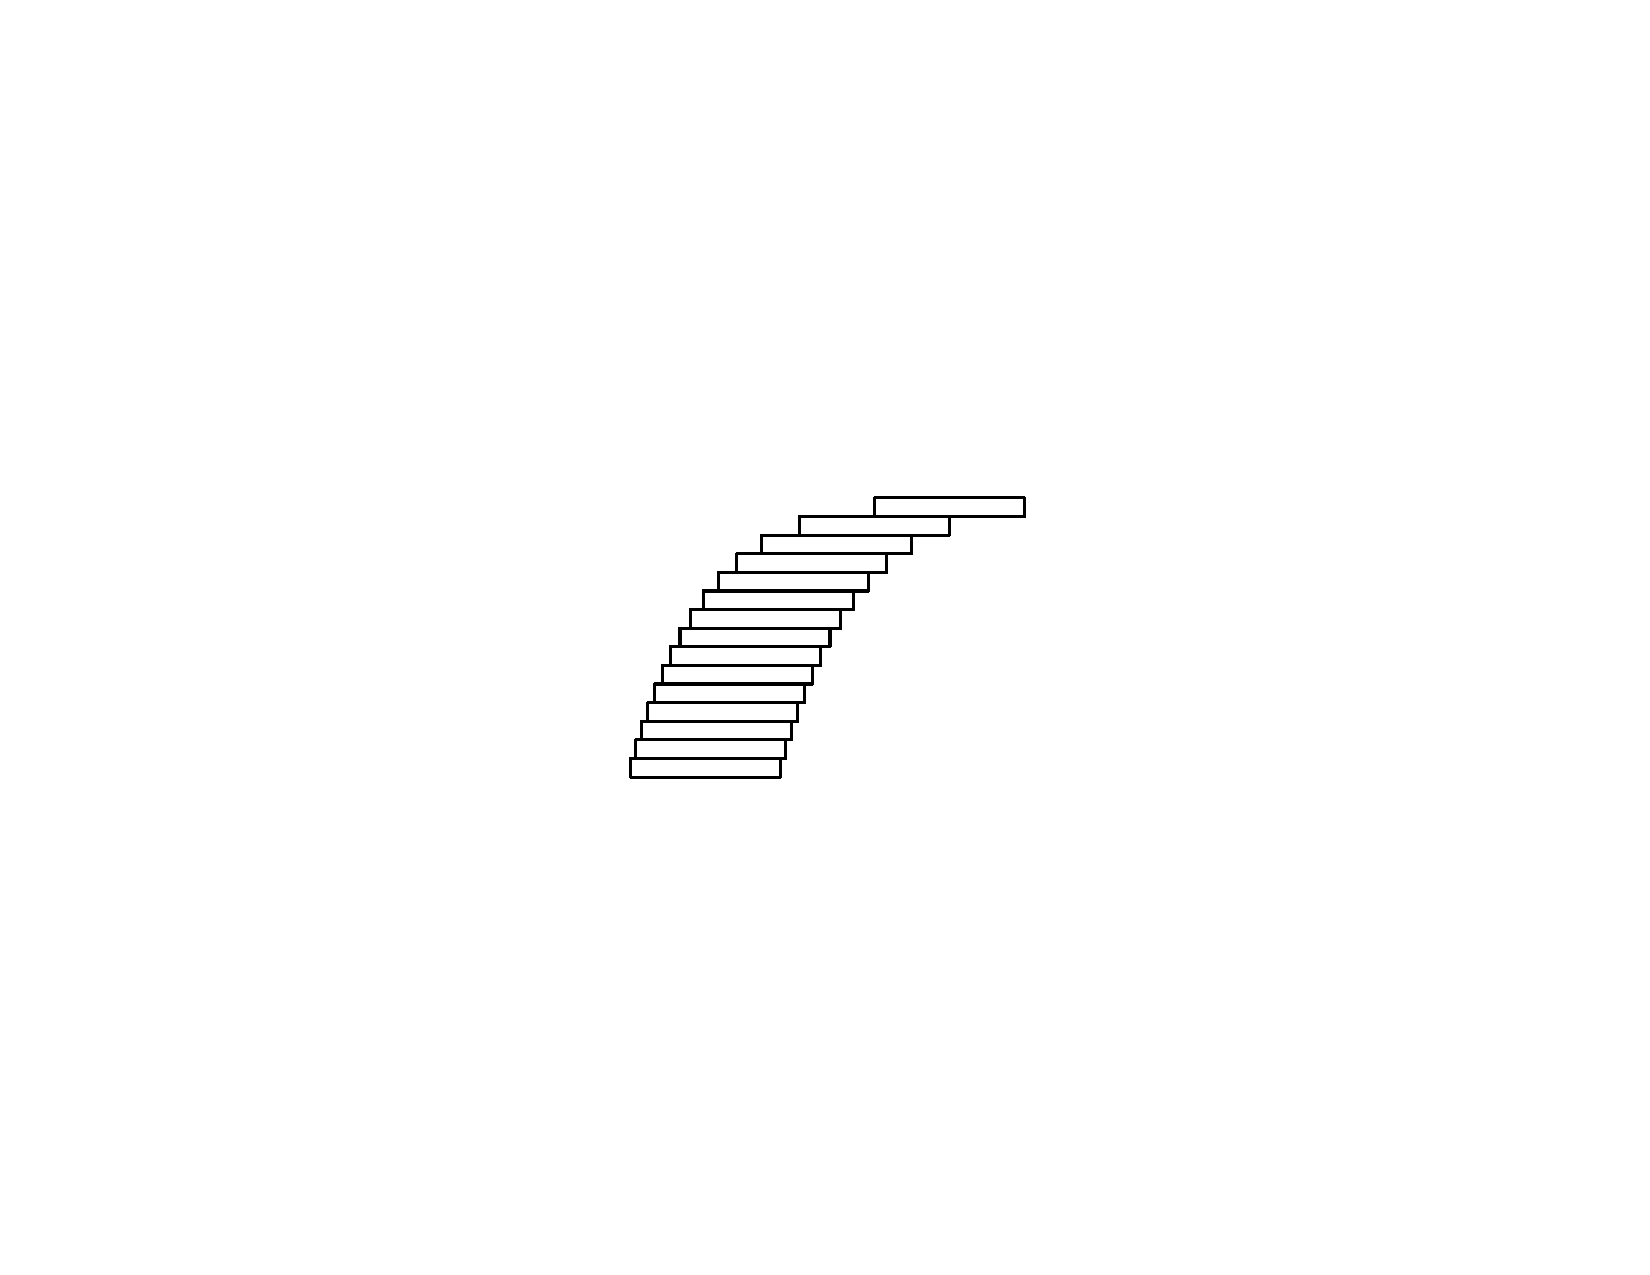
\includegraphics{blocks.pdf}
\end{center}
\noindent
The rightmost block is $1/2$ inch to the right of the block under it;
the second block from the top is $1/4$ inch to the right of the block
underneath it, the third block from the top is $1/6$ inch to the right
of the block under it.  In general, the $n^{\mbox{\underline{th}}}$ block from the top is
$1/(2n)$ inches to the right of the $(n+1)^{\mbox{\underline{th}}}$ block.
\begin{description}
\item[Part (a)] Prove that this structure will not fall over, no
matter how many blocks are used.
\item[Part (b)] As I use more and more blocks, how far to the right of the bottom block will the top block be?
\end{description}
\end{problem}

\begin{problem}[3]
Give an example of sequences $\{ a_n \}$ and $\{ b_n \}$ so that
$\displaystyle\sum_{n=1}^\infty a_n$ and
$\displaystyle\sum_{n=1}^\infty b_n$ both diverge, but
$\displaystyle\sum_{n=1}^\infty \left( a_n + b_n \right)$ converges.
\end{problem}

\begin{problem}[2]
Does $\displaystyle\sum_{n=10}^\infty \frac{3}{n - 9}$ converge or
diverge?  Why or why not?
\end{problem}


\begin{problem}[4]
Dramatically, Alice and Bob are driving very slow cars, and they are
on a collision course, heading toward each other at the constant speed
of 5~mph.  Alice and Bob are currently 5~miles apart, when a bee
(travelling at 10~mph) begins to fly from Alice's bumper, to Bob's
bumper, back to Alice's bumper, back to Bob's bumper, and so
on---until that fateful moment when the bee will be squished.
\textbf{How far will the bee travel in its journey?}
\begin{description}
\item[Part (a)] Write down a \textit{geometric series} giving the
total distance the bee travels.
\item[Part (b)] Use a trick to compute the answer instantly (i.e.,
use the speed of the bee, and the time for which the bee is flying, to calculate
the value of the geometric series).
\end{description}

\end{problem}



\end{document}
